% Grossmont College -- Chem 141 Lab 1
% Cameron Carroll
% February 2014


\documentclass[fleqn,titlepage]{article}

\renewcommand*\rmdefault{ppl}

\usepackage[version=3]{mhchem} % Package for chemical equation typesetting
\usepackage{tabu}
\usepackage{wasysym}
\usepackage{listings}
\usepackage{scrextend}
\lstset{language=Matlab}

% set 1" margins on 8.5" x 11" paper
% top left is measured from 1", 1"
\topmargin 0in
\oddsidemargin 0in
\evensidemargin 0in
\headheight 0in
\headsep 0in
\topskip 0in
\textheight 9in
\textwidth 6.5in

\usepackage{graphicx} % Required for the inclusion of images

\setlength\parindent{0pt} % Removes all indentation from paragraphs

\renewcommand{\labelenumi}{\alph{enumi}.} % Make numbering in the enumerate environment by letter rather than number (e.g. section 6)

%\usepackage{times} % Uncomment to use the Times New Roman font

%----------------------------------------------------------------------------------------
% DOCUMENT INFORMATION
%----------------------------------------------------------------------------------------

\begin{document}

\begin{titlepage}
  \mbox{}\\[1.25cm]
  \textbf{\LARGE Cameron Carroll \\ Grossmont College}\\[2.25cm]
  \begin{center}
    \textbf{\huge Experiment 2: \\ Conductivity and Net Ionic Equations}\\[2.50cm]
  \end{center}
  \textbf{\LARGE Professor: Martin Larter \\ Chemistry 141-0692} \\
  \vfill
  \center{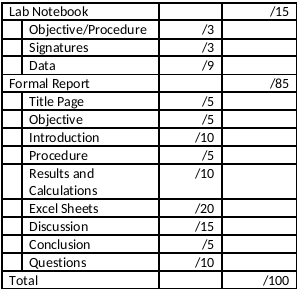
\includegraphics{./rubric_stdev}}
  \center{\textbf{\LARGE Performed --} {\LARGE February 6 \& 11, 2014}}
  \center{\textbf{\LARGE Submitted --} {\LARGE February 20, 2014}}
\end{titlepage}

%----------------------------------------------------------------------------------------
% SECTION 1
%----------------------------------------------------------------------------------------
\section*{Objective}
  \paragraph{} The goals of this experiment include determining the type of bonding of a substance based on observations of its conductivity. Also we observe how conductivity changes with the addition of a solvent, both with polar and nonpolar solutes. We then try to find a correlation between conductivity and reaction rate. Finally, we observe how conductivity changes as a reaction proceeds.


%----------------------------------------------------------------------------------------
% SECTION 2
%----------------------------------------------------------------------------------------
\section*{Introduction}
  \paragraph{} 

%----------------------------------------------------------------------------------------
% SECTION 3
%----------------------------------------------------------------------------------------
\newpage
\section*{Procedure}
\begin{itemize}
  \item  \textbf{Referenced From:} \\
    \begin{addmargin}[1em]{1em}
      Lehman, J. (Et alia), `Measuring Density with Different Types of Glassware' \\
      Grossmont College, Chemistry 141 Lab Manual, 6th edition, pp 1-13 \\
      El Cajon, California
    \end{addmargin}
\end{itemize}

%----------------------------------------------------------------------------------------
% SECTION 4
%----------------------------------------------------------------------------------------
\section*{Discussion}
  \paragraph{}
, 
%----------------------------------------------------------------------------------------
% SECTION 6
%----------------------------------------------------------------------------------------
\section*{Conclusion}
  \paragraph{} 

\end{document}